\subsection{Mediator}

Este \textit{pattern} é utilizado para reduzir a complexidade de comunicação entre várias classes. É fornecido uma classe \textit{Mediator} que é o mediador que lida com todas as comunicações entre diferentes objetos e facilita a manutenção do código.
Existe uma baixa junção entre os objetos, evitando que estes façam referências uns aos outros de forma explícita, permitindo assim utilizar interações de forma independente.\\

\textbf{Problema}

Como se permite que um grupo de objetos comuniquem entre si sem que haja junção entre eles?\\

\textbf{Solução}

\begin{figure}[!h]
\centering
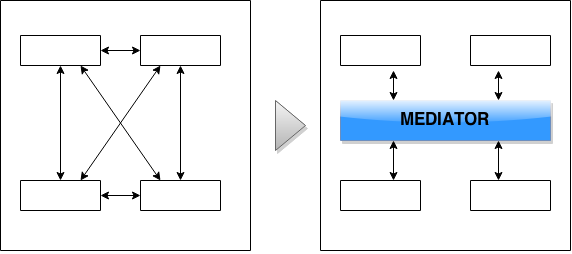
\includegraphics[scale=0.7]{img/mediator-solucao}
\caption{Proposta de solução ao problema anterior}
\end{figure}

Ao se introduzir um \textit{Mediator} (conhece todos os participantes), os objetos podem comunicar sem se conhecer, ignorando assim a existência de outros objetos no sistema.

A interface \textit{Mediator} é utilizada para iniciar a comunicação com as classes e receber pedidos dos objetos, enviando o mesmo para um destino.\\


\textbf{Participantes}

\begin{itemize}
  \item Mediator - É definida uma interface para a comunicação entre os objetos \textit{Colleague}.

  \item ConcreteMediator - Sabe da existência das classes \textit{Colleague} e guarda uma referência a estes objetos. Implementa a comunicação e transferência de mensagens entre as classes \textit{Colleague}.

  \item Classes Colleague - Tem uma referência ao objeto \textit{Mediator}. Comunica com este sempre que necessário. Caso contrário, comunica com um \textit{Colleague}.\\
\end{itemize}

\textbf{Colaboração}

As classes \textit{Colleague} enviam e recebem pedidos do \textit{Mediator}. Cabe a este implementar um comportamento colaborativo ao tratar e redireccionar os pedidos para os objetos \textit{Colleague} responsáveis.\\

\textbf{Implementação}

\begin{figure}[!h]
\centering
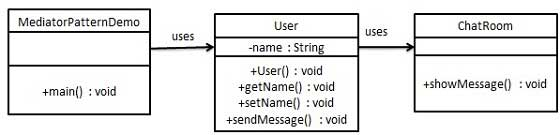
\includegraphics[scale=0.7]{img/mediator_diagrama}
\caption{Diagrama de classe}
\end{figure}

Nesta implementação os utilizadores enviam mensagens entre si para comunicarem, e é responsabilidade da classe \textit{ChatRoom} mostrar as mensagens a todos os utilizadores no sistema.

Já o objeto \textit{MediatorPatternDemo} utiliza as classes \textit{User} para mostrar as comunicações entre elas.\\


\textbf{Vantagens}

\begin{itemize}
  \item Separação entre os participantes da rede de comunicação.
  \item Remoção de relacionamentos muitos para muitos, sendo substituídos por relações um para muitos.
  \item As regras de comunição está centrada no \textit{mediator}, logo podem ser feitas alterações sem mexer nos colaboradores.\\
\end{itemize}

\textbf{Desvantagens}

\begin{itemize}
  \item Pode ser uma fonte de problemas de desempenho a centralização existente nos sistemas, em caso de falha.
  \item Os \textit{mediators} podem tornar-se bastante complexos.
\end{itemize}
